\chapter{Experiments}
\label{chap:experiments}
This chapter presents how the experiments were conducted.
\todo{parameters? check what is mentioned in earlier chapters and include those}
50k steps

\todo{Losses in 4 Bilder neben und untereinander. Die Eval ineinnander und Training metrics weglassen.}


\section{Mastermind}
\label{sec:ex_mastermind}

For the Mastermind environment, the size of the action space covers $6^4$ units, each of which covers a possible colour combination, and the observation space is covered by $2 \times 4$ observations, one row for the guess by the codebreaker and the other for feedback by the codemaker. Additionally, the observation includes another list, which covers all valid actions for the current state of the environment. Based on the feedback, this list will be adjusted at each iteration and will only retain actions that score equally to, or better, than the current action. This ensures, that the agent is not making \textit{worse} guesses  and takes the feedback into consideration for its next move. The reward is simple, if the agent was able to break the code, it receives a reward of \textit{1}, if not, the agent receives a reward of \textit{-1}. An episode ends after 10 steps.

\subsection{Results}
Figure \ref{fig:dqn_tderr} shows the TD error for 50.000 training steps. It is visible that the DQN agent is already minimizing its loss in the very early stages of its training and the loss is fluctuating around 0.55, with 0.08 being the lowest value and 0.88 the highest. However, due to its extreme lowness, it might be an outlier and 0.23 could be considered the lowest value. All three extremes appear before passing 10.000 training steps, so it might be sufficient to run only those number of training steps, or less, to achieve similar results. 

\begin{figure}[H]
	\centering
	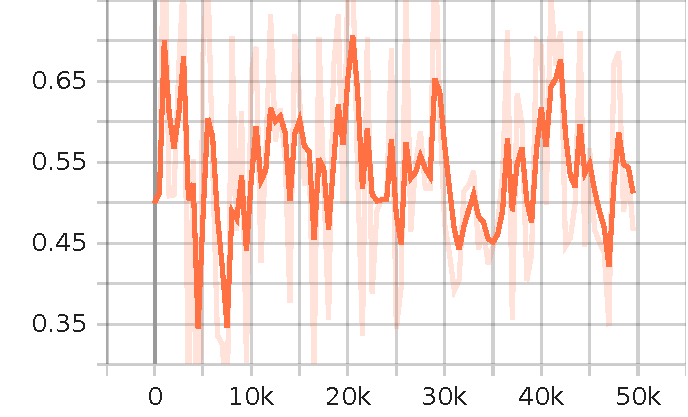
\includegraphics[scale=.75]{images/stats/dqn_50k/Losses_td_loss}
	\caption[DQN loss]{Loss of the DQN agent in Mastermind. The x-axis displays the number of training steps and the y-axis the loss value.}
	\label{fig:dqn_tderr}
\end{figure}

The training metrics of the agent suggests the previous observation as well. The values for the average return and length of an episode are each marginally close, the return between around -2 and -3, and the episode number between around 4 and 5, as seen in figure \ref{fig:dqn_train}. The average episode length, as well as average return, are fluctuating between those values; with no significant increase, or decrease, of performance regarding training duration.


\begin{figure}[H]
	\centering
	\subfloat[Average episode length]{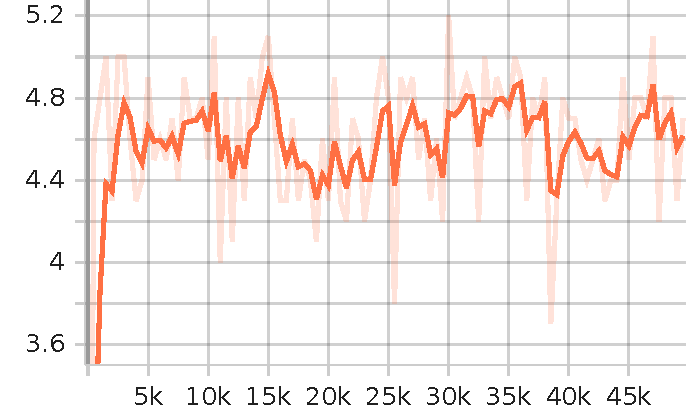
\includegraphics[scale=.6]{images/stats/dqn_50k/Metrics_Train_AverageEpisodeLength} }
	\qquad
	\subfloat[Average return]{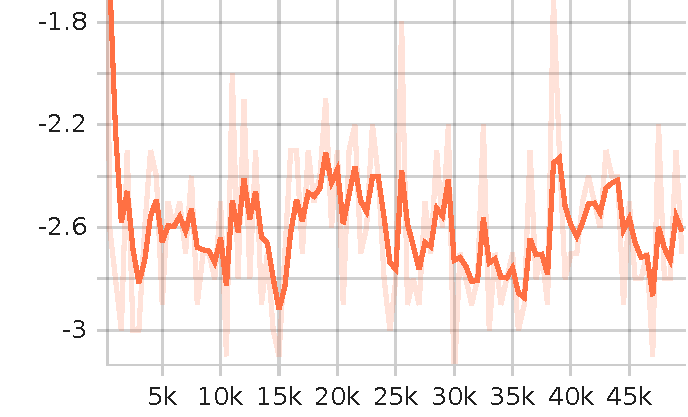
\includegraphics[scale=.6]{images/stats/dqn_50k/Metrics_Train_AverageReturn} }
	\caption[DQN Training]{Training metrics DQN. In both diagrams the x-axis displays the number of evaluation steps. The y-axis displays the average episode number in (a) and the average return in (b).}	
	\label{fig:dqn_train}
\end{figure}


The evaluation of the agent in figure \ref{fig:dqn_eval} confirms the observation that 10.000 training steps would be sufficient. The metrics show similar value to the training. Again, they fluctuating within the same range but generally, over time, no significant increase, or decrease, in performance.

\begin{figure}[H]
	\centering
	\subfloat[Average episode length]{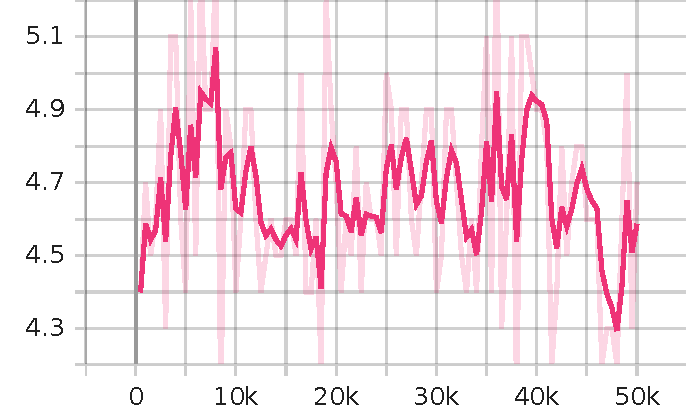
\includegraphics[scale=.6]{images/stats/dqn_50k/Metrics_Eval_AverageEpisodeLength} }
	\qquad
	\subfloat[Average return]{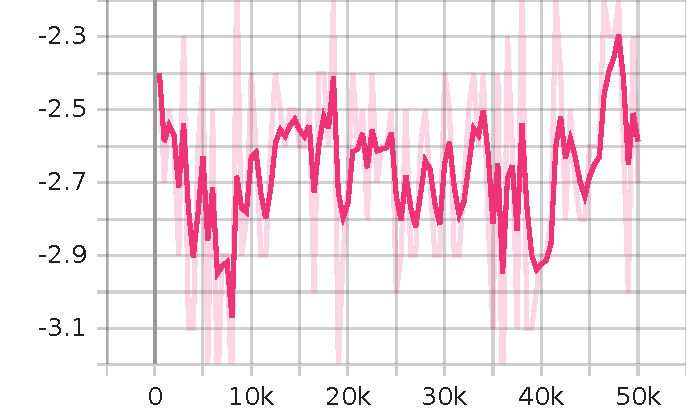
\includegraphics[scale=.6]{images/stats/dqn_50k/Metrics_Eval_AverageReturn} }
	\caption[DQN Evaluation]{Evaluation metrics DQN. The labels of the axes are the same as in figure \ref{fig:dqn_train}.}	
	\label{fig:dqn_eval}
\end{figure}

\todo{insert combined training and eval metrics}
Figure X shows the training and evaluation metrics of all four agents combined. All agents show quite similar results, as seen in the figure. The reason for this result is that all agents mask invalid actions with the same method, i.e. actions that do not result in at least the same number of correctly guessed color combinations are not executed. Thus, resulting in breaking the code with each agent on average with \textbf{4.6} guesses. Complementary, the individual results of the remaining agents can be found in appendix \ref{chap:app_exp}.

\section{Battleship}
\label{sec:ex_battleship}
The environment of the Battleship contains an action space of $10^2$ actions and an observation space by the size of $10 \times 10$, resulting in 100 cells on the board. The values for the cells in the observation are bounded between minus one and one: 

\begin{itemize}

	\item{-1 for a miss}
	\item{0 for unkown, i.e. unexplored cell}
	\item{1 for a hit}

\end{itemize}
This is what the agent is receiving. There is another list that includes the complete placements of the ships, however, this is only used for rendering purposes and validation purposes. \todo{Reward?, Action masking?}